
\documentclass[a4paper,11pt]{article}

\usepackage[utf8]{inputenc}
\usepackage[T1]{fontenc}
\usepackage[italian]{babel}
\usepackage{amsmath,amssymb}
\usepackage{siunitx}
\usepackage[a4paper, top=1cm, bottom=1cm, left=1.5cm, right=1.5cm]{geometry}
\usepackage{graphicx}
\usepackage{enumitem}
\usepackage{pgfplots}
\usepackage{float}
\pgfplotsset{compat=1.18}

\geometry{margin=2.2cm}
\sisetup{per-mode=symbol}

\title{Esercizio 134 pag. 290 -- Cutnell \& Johnson}
\author{}
\date{}

\begin{document}
\maketitle
\section{Esercizio nr 134 pag 290}
La figura mostra l’andamento dell’accelerazione di una motocicletta che ha una velocità iniziale di $28\ \text{km/h}$.
Una seconda motocicletta, con la stessa velocità iniziale, nello stesso intervallo di tempo compie un moto analogo, in cui però il valore della terza accelerazione è scambiato con il valore della prima.
\begin{figure}[H]
  \centering
  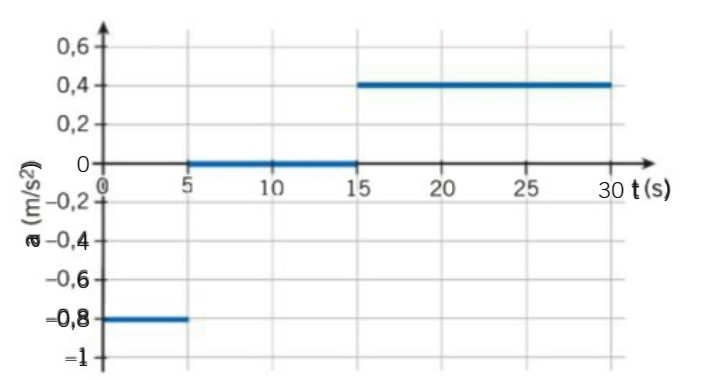
\includegraphics[width=0.5\linewidth]{../../immagini/grafico_accelerazioneEs131pag290.jpg}
  \caption{Andamento dell’accelerazione in funzione del tempo}
  \label{fig:grafico-acc}
\end{figure}
\medskip
\begin{itemize}
\item Calcola la differenza tra lo spazio percorso dalla seconda motocicletta
      e quello percorso dalla prima;
\item determina prima l’espressione algebrica di questa differenza in funzione
      delle accelerazioni e degli istanti di tempo;
\item inserisci solo alla fine i dati numerici.
\end{itemize}
\newpage

\section{Analisi del contesto}
Ci sono due motociclette, che indicheremo con A e B, il cui moto è descritto dal grafico  dell'accelerazione 1 e 2 da cui si evince che è un moto vario.
Da una prima analisi si puo osservare che nel primo e nel terzo tratto si tratta di un MRUA con $a\neq 0 $
\subsection{Strategia generale}
Analizziamo lo spazio percorso dalle due motociclette in modo separato e poi facciamo la differenza dei 2 percorsi.
\subsection{Analisi del percorso della motocicletta A}
Il grafico sottostante rappresenta l'andamento dell'accelerazione in funzione del tempo.

\begin{figure}[h]
\centering
\begin{tikzpicture}
\begin{axis}[
    axis lines=middle,
    xlabel={$t\;(\si{s})$},
    ylabel={$a\;(\si{m/s^2})$},
    xmin=0, xmax=32,
    ymin=-1, ymax=1,
    xtick={0,5,15,30},
    ytick={-0.8,-0.4,0,0.4,0.8},
    width=12.5cm,
    height=5.8cm,
    grid=both,
    minor tick num=1
]
\addplot[line width=2] coordinates {(0,-0.8) (5,-0.8)};
\addplot[line width=2] coordinates {(5,0) (15,0)};
\addplot[line width=2] coordinates {(15,0.4) (30,0.4)};
\end{axis}
\end{tikzpicture}
\caption{Andamento dell’accelerazione in funzione del tempo}
\label{fig:acc}
\end{figure}

Il moto si sviluppa in 3 tratti:
\begin{enumerate}
\item  $t \in [0,5]$\ \text{s}, \quad $a = a_1$ \quad \text{(M.R.U.A.)}.
\item  $t \in [5,15]$\ \text{s}, \quad $a = 0$ \quad \text{(M.R.U.)}. 
\item  $t \in [15,20]$\ \text{s}, \quad $a = a_3$ \quad \text{(M.R.U.A.)}.
\end{enumerate}
Nello specifico nei tre tratti i dati sono: 
\begin{enumerate}
\item $a_1 = -0{,}8\ \text{m/s}^2$ (M.R.U.A.) per una durata $T_1 = 5\ \text{s}$, con velocità iniziale $v_0 = 28\ \text{km/h} \approx 7{,}8\ \text{m/s}$.

\item $a_2 = 0$ (M.R.U.) per una durata $T_2 = 10\ \text{s}$,  
      con velocità costante pari a quella in uscita dal tratto 1.

\item $a_3 = 0{,}4\ \text{m/s}^2$ (M.R.U.A.) per una durata $T_3 = 15\ \text{s}$, con velocità iniziale pari a quella del tratto precedente.
\end{enumerate}
\newpage

\subsection{Analisi del percorso della motocicletta B}
L'analisi della motocicletta B è del tutto analoga alla precedente.
\begin{figure}[h]
\centering
\begin{tikzpicture}
\begin{axis}[
    axis lines=middle,
    xlabel={$t\;(\si{s})$},
    ylabel={$a\;(\si{m/s^2})$},
    xmin=0, xmax=32,
    ymin=-1, ymax=1,
    xtick={0,5,15,30},
    ytick={-0.8,-0.4,0,0.4,0.8},
    width=12.5cm,
    height=5.8cm,
    grid=both,
    minor tick num=1
]
\addplot[line width=2] coordinates {(0,0.4) (5,0.4)};
\addplot[line width=2] coordinates {(5,0) (15,0)};
\addplot[line width=2] coordinates {(15,-0.8) (30,-0.8)};
\end{axis}
\end{tikzpicture}
\caption{Andamento dell’accelerazione in funzione del tempo}
\label{fig:acc2}
\end{figure}

Quindi, per la motocicletta B nei vari tratti si ha:
\begin{enumerate}
\item $a'_1 = a_3 = 0{,}4\ \text{m/s}^2$ per una durata $T_1 = 5\ \text{s}$.

\item $a'_2 = a_2 = 0$ per una durata $T_2 = 10\ \text{s}$.

\item $a'_3 = a_1 = -0{,}8\ \text{m/s}^2$ per una durata $T_3 = 15\ \text{s}$.
\end{enumerate}


\section{Svolgimento}
Passiamo quindi a calcolare gli spazi percorsi, prima per la motocicletta A e poi per la motocicletta B.
\\
\subsection{Formule da ricordare - cenni teorici}
\begin{itemize}
\item per il moto rettilineo uniformemente accelerato (M.R.U.A.):
\[
s(t) = s_0 + v_0 t + \frac{1}{2} a t^2,
\qquad
v(t) = v_0 + a t;
\]

\item per il moto rettilineo uniforme (M.R.U.):
\[
s(t) = s_0 + v_0 t.
\]
\end{itemize}
\medskip
\text{NB: per entrambi i percorsi si sottintende $s_0 = 0$.} 

\subsection{Equazione del percorso della motocicletta A}
Andiamo quindi a determinare le equazioni che descrivono gli spazi percorsi dalle 2 motociclette
\subsubsection{Tratto 1:}
\[
\Delta s_1 = v_0 T_1 + \frac{1}{2} a_1 T_1^2
\]

La velocità in uscita dal tratto $T_1$ si calcola utilizzando la prima equazione del moto
rettilineo uniformemente accelerato:
\[
v(t) = v_0 + a t.
\]
Pertanto:
\[
v_{01} = v_0 + a_1 T_1,
\]
dove $v_{01}$ rappresenta la velocità finale del tratto 1.

\subsubsection{Tratto 2:}
Il secondo tratto è un moto rettilineo uniforme (M.R.U.), in cui la velocità è pari
a quella in uscita dal tratto precedente. Pertanto:
\[
\Delta s_2 = v_{0,1}\,T_2 = (v_0 + a_1 T_1)\,T_2.
\]
\subsubsection{Tratto 3:}
Il terzo tratto è un moto rettilineo uniformemente accelerato (M.R.U.A.), in cui
la velocità iniziale è uguale a quella del tratto precedente. Lo spazio percorso è quindi:
\[
\Delta s_3 = v_{01}\,T_3 + \frac{1}{2} a_3 T_3^2
           = (v_0 + a_1 T_1)\,T_3 + \frac{1}{2} a_3 T_3^2.
\]
\subsubsection{Percorso totale}
Lo spazio totale percorso dalla motocicletta A è quindi:
\[
\begin{aligned}
S_A &= \Delta S_1 + \Delta S_2 + \Delta S_3 \\[4pt]
&= v_0 T_1 + \frac{1}{2} a_1 T_1^2 
   + (v_0 + a_1 T_1) T_2 
   + (v_0 + a_1 T_1) T_3 
   + \frac{1}{2} a_3 T_3^2 \\[6pt]
&= v_0 T_1 + \frac{1}{2} a_1 T_1^2 
   + v_0 T_2 + a_1 T_1 T_2 
   + v_0 T_3 + a_1 T_1 T_3 
   + \frac{1}{2} a_3 T_3^2 \\[6pt]
&= v_0 (T_1 + T_2 + T_3)
   + a_1 \left( \frac{1}{2} T_1^2 + T_1 T_2 + T_1 T_3 \right)
   + a_3 \left( \frac{1}{2} T_3^2 \right).
\end{aligned}
\]
Possiamo concludere affermando che:
\[
S_A = v_0 (T_1 + T_2 + T_3)
      + a_1 \left( \frac{1}{2} T_1^2 + T_1 T_2 + T_1 T_3 \right)
      + a_3 \left( \frac{1}{2} T_3^2 \right).\tag{1}
\]

\section*{Percorso della motocicletta B}
In modo del tutto analogo possiamo scrivere l'equazione della motocicletta B dove sappiamo che:
\begin{enumerate}
\item $a'_1 = a_3 = 0{,}4\ \text{m/s}^2$ per una durata $T_1 = 5\ \text{s}$.

\item $a'_2 = a_2 = 0$ per una durata $T_2 = 10\ \text{s}$.

\item $a'_3 = a_1 = -0{,}8\ \text{m/s}^2$ per una durata $T_3 = 15\ \text{s}$.
\end{enumerate}
\subsubsection{Percorso totale}
\[
S_B = v_0 (T_1 + T_2 + T_3)
      + a'_1 \left( \frac{1}{2} T_1^2 + T_1 T_2 + T_1 T_3 \right)
      + a'_3 \left( \frac{1}{2} T_3^2 \right).
\]
Sostituendo con le equivalenti accelerazioni otteniamo l'equazione della motocicletta B nelle tre accelerazioni iniziali:
\[
S_B = v_0 (T_1 + T_2 + T_3)
      + a_3 \left( \frac{1}{2} T_1^2 + T_1 T_2 + T_1 T_3 \right)
      + a_1 \left( \frac{1}{2} T_3^2 \right). \tag{2}
\]
\section{Differenza dei due percorsi $(S_B - S_A)$}
Dalle equazioni (1) e (2) possiamo quindi ottenere:
\[
\begin{aligned}
S_B - S_A
&= v_0 (T_1 + T_2 + T_3)
 + a_3 \left( \frac{1}{2} T_1^2 + T_1 T_2 + T_1 T_3 \right)
 + a_1 \left( \frac{1}{2} T_3^2 \right) \\[6pt]
&\quad - v_0 (T_1 + T_2 + T_3)
 - a_1 \left( \frac{1}{2} T_1^2 + T_1 T_2 + T_1 T_3 \right)
 - a_3 \left( \frac{1}{2} T_3^2 \right) \\[6pt]
&= (a_3 - a_1)
   \left( \frac{1}{2} T_1^2 + T_1 T_2 + T_1 T_3 \right)
 + (a_1 - a_3)
   \left( \frac{1}{2} T_3^2 \right) \\[6pt]
&= (a_3 - a_1)
   \left( \frac{1}{2} T_1^2 + T_1 T_2 + T_1 T_3
          - \frac{1}{2} T_3^2 \right).
\end{aligned}  
\]
\subsubsection{Equazione generale della differenza }
\[
S_B - S_A = (a_3 - a_1)
   \left( \frac{1}{2} T_1^2 + T_1 T_2 + T_1 T_3
          - \frac{1}{2} T_3^2 \right).\tag{3}
\]
dove, per i valori numerici dell'esercizio:
\[
a_1=-0.8~\si{m/s^2},\qquad a_3=+0.4~\si{m/s^2}, \qquad T_1=5~\si{s},\qquad T_2=10~\si{s},\qquad\ T_3 = 15~\si{s}.
\]
Sostuendo quindi i valori nell'equazione (3) otteniamo:
\[
\begin{aligned}
S_B - S_A
&= \left[ 0{,}4\,\frac{\text{m}}{\text{s}^2}
          - \left(-0{,}8\,\frac{\text{m}}{\text{s}^2}\right) \right]
   \left( \frac{1}{2}\,5^2 + 5\cdot 10 + 5\cdot 15 - \frac{1}{2}\,15^2 \right) \\[6pt]
&= \left( 1{,}2\,\frac{\text{m}}{\text{s}^2} \right)
   \left( 12{,}5 + 50 + 75 - 112{,}5 \right)\,\text{s}^2 \\[6pt]
&= 1{,}2\,\frac{\text{m}}{\text{s}^2} \cdot 25\,\text{s}^2
 = 30\,\text{m}.
\end{aligned}
\]
\[
S_B-S_A = 1.2\cdot 25 = 30~\si{m}.
\]

\section{Conclusione}
Dall’analisi dei due moti si evince che la motocicletta B percorre $30\,\text{m}$ in più rispetto alla motocicletta A. Tale risultato si giustifica dal fatto che la motocicletta B,
accelerando all’inizio del moto, mantiene una velocità maggiore per un intervallo di tempo più lungo rispetto alla motocicletta A.
\[
\boxed{S_B - S_A = 30~\si{m}}
\]
\newpage
\section{Nota didattica / metodologica: Lo spazio nel moto a tratti}
Quando analizziamo un moto in cui l'accelerazione cambia (moto uniformemente accelerato a tratti), dobbiamo calcolare lo spostamento $\Delta s$ per ogni singolo intervallo.
Un errore comune è pensare che lo spostamento dipenda dalla differenza dei quadrati dei tempi assoluti
$(t_2^2 - t_1^2)$.
In realtà, si deve usare il quadrato della durata dell'intervallo $(\Delta t)^2$.

\subsection{La formula per singolo tratto}

Per un intervallo di tempo che inizia al tempo $t_1$ e finisce al tempo $t_2$, definiamo la durata come:
\[
\Delta t = t_2 - t_1.
\]

Se all'istante $t_1$ l'oggetto ha una velocità $v_1$ e un'accelerazione costante $a$, lo spostamento compiuto in quell'intervallo è:
\[
\Delta s = v_1 \Delta t + \frac{1}{2} a (\Delta t)^2.
\]

\subsection{Perché non si usa $(t_2^2 - t_1^2)$?}

Supponiamo di voler calcolare la posizione finale $x(t_2)$ partendo dalla posizione iniziale $x(0)=0$ con velocità iniziale $v_0=0$ e accelerazione costante $a$.
In questo caso particolare:
\[
x(t_2) = \frac{1}{2} a t_2^2,
\qquad
x(t_1) = \frac{1}{2} a t_1^2.
\]

Quindi lo spostamento sarebbe:
\[
\Delta s = x(t_2) - x(t_1) = \frac{1}{2} a (t_2^2 - t_1^2).
\]

Attenzione però: questa formula della ``differenza di quadrati'' funziona solo se l'accelerazione $a$ è rimasta la stessa fin dall'istante zero e la velocità iniziale era nulla.

\subsection{Il segreto: la velocità iniziale del tratto}

Nel nostro problema, l'accelerazione cambia ad ogni tratto.
Questo significa che all'inizio di ogni nuovo intervallo, la motocicletta ha già una velocità ``ereditata'' dal tratto precedente.\\
\\
Usando la durata dell'intervallo $\Delta t$, trattiamo ogni pezzetto come un nuovo inizio:
\begin{itemize}
\item $\Delta t$: quanto tempo è durato lo sforzo del motore in quel tratto?
\item $v_1$: a che velocità andavo quando ho iniziato quel tratto?
\end{itemize}

In sintesi: per non sbagliare mai, ``resetta'' il cronometro all'inizio di ogni intervallo e usa sempre il quadrato del tempo trascorso in quel pezzetto $(\Delta t)^2$, ricordandoti di sommare l'effetto della velocità iniziale di quel tratto $(v_1 \cdot \Delta t)$.


\end{document}
